\documentclass[tikz]{standalone}
\usepackage{amsmath}
\usetikzlibrary{calc}
\definecolor{bg}{HTML}{171D2B}
\definecolor{accent}{HTML}{F7B538}
\begin{document}
\pagecolor{bg}
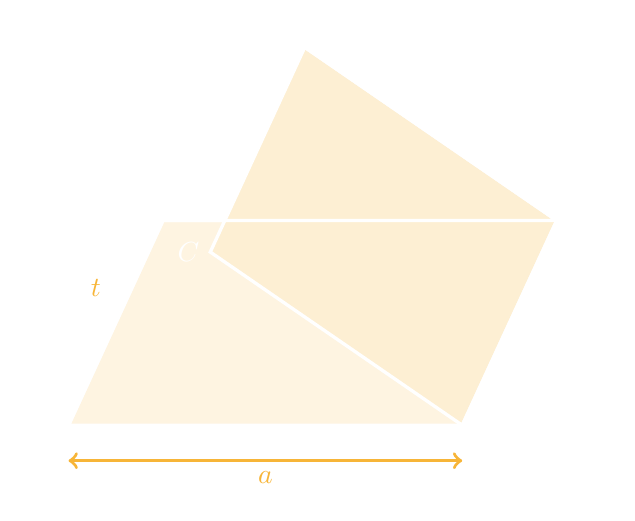
\begin{tikzpicture}[line width=1.2pt, x=1cm, y=1cm]
  \color{white}
  % Proyeksi oblique: sumbu z digambar miring ke kanan-atas
  % alas segitiga ABC di bidang bawah, A'B'C' di bidang atas (digeser vektor (1.2,2.6))
  \coordinate (A) at (0,0);
  \coordinate (B) at (5,0);
  \coordinate (C) at (1.8,2.2);
  \coordinate (A2) at ($(A)+(1.2,2.6)$);
  \coordinate (B2) at ($(B)+(1.2,2.6)$);
  \coordinate (C2) at ($(C)+(1.2,2.6)$);
  % sisi tenggelam: AC (tertutup badan prisma) -> putus-putus
  \draw[white, dashed] (A) -- (C);
  \draw[white, dashed] (C) -- (C2);
  % sisi tampak
  \draw[fill=accent!30, draw=white] (A) -- (B) -- (C) -- cycle;
  \draw[fill=accent!15, draw=white] (A) -- (B) -- (B2) -- (A2) -- cycle;
  \draw[fill=accent!22, draw=white] (B) -- (C) -- (C2) -- (B2) -- cycle;
  \draw[white] (A2) -- (B2) -- (C2) -- (A2);
  \draw[white] (A) -- (A2);
  \draw[white] (B) -- (B2);
  % label titik
  \node[below left]  at (A) {\color{white}$A$};
  \node[below right] at (B) {\color{white}$B$};
  \node[left]        at (C) {\color{white}$C$};
  \node[above left]  at (A2) {\color{white}$A'$};
  \node[above right] at (B2) {\color{white}$B'$};
  \node[right]       at (C2) {\color{white}$C'$};
  % panjang rusuk alas
  \draw[accent, <->] (0,-0.45) -- (5,-0.45) node[midway, below] {\color{accent}$a$};
  % tinggi prisma = rusuk tegak AA'
  \node[above left, accent] at (0.55,1.5) {\color{accent}$t$};
\end{tikzpicture}
\end{document}
